\chapter{Interweave System}
\label{chap:IS}
\index{Interweave System}

\section{Introduction}
Sharing principle -- Orthogonal in time domain 

\subsection{Detection/Sensing}
Primary user detection \\ 
\begin{itemize}
\item Energy detection
\item Matched filtering
\item Cyclostationary detection
\item Feature based detection
\end{itemize}
Compare the \ac{ROC} for different detection principle 

%\subsection{Energy detection}
%\subsubsection{Determining threshold} 
%\subsubsection{Path loss}
%\subsubsection{Fading}
%Rayleigh fading \\
%Nakagammi-$m$ fading

%\section{Single \ac{CR}}
%Briefly CFAR vs CDR
%Why determining CD is a problem?
%\begin{itemize}
%\item Knowledge of the channel 
%\item Difficult to tract the distribution of the detection probability analytically 
%\end{itemize}

\section{Performance Characterization}
\subsection{System Model}
\subsection{Sensing-Throughput Tradeoff}
%\subsection{Imperfect channel estimation}
%\subsection{Noise uncertainty}
%\subsection{Mixture models}
Combating noise uncertainty, where the parameters of the density representing the two Hypothesis are estimated jointly to characterize the \ac{ROC} and determine threshold. 

\section{Cognitive sensing}
\subsection{Markov model}
Estimation of modal parameters
\ac{MLE}
\subsubsection{Complete data set}
\subsubsection{Incomplete data set}
\ac{EM}\cite{Kaushik_WCNC} 

\section{Cognitive relay networks ?}
\subsection{System model}
Exclusion zone
%This chapter gives an overview of the platforms and their components that are used in this work. The chapter starts with a general overview of SDR platforms and presents the different used platforms in detail. Furthermore, the integration in the development flow is shown, which was introduced in section \ref{sec:mbd}.
%
%\section{SDR Platforms in General}
%
%Software Defined Radio is associated with digital signal processing, implemented on reconfigurable processors. The interface to the analog world is done by the \ac{ADC} and \ac{DAC}, which are as close as possible to the antenna. It should be highlighted that reconfigurable digital signal processing is the core part of any SDR. The RF signals in the physical analog world are on high frequencies at low power and the \ac{ADC} sampling rate, dynamic range and power consumption are limited \cite{reed_SR}. Therefore, the RF front end should only extract a dedicated frequency band of interest and convert it into a signal suitable for the \ac{ADC}. After AD conversion the digital signal processing is in dependence on the underlying digital hardware. This scheme is represented in figure \ref{fig:SDR_platform}.
%
%\begin{figure}
%	\centering
%		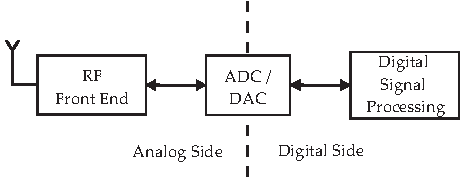
\includegraphics{../kapitel03/figures/SDR_platform.pdf}
%	\caption{Structure of a general SDR platform}
%	\label{fig:SDR_platform}
%\end{figure}
%
%
%\subsection{RF Front Ends in SDR}
%\index{RF front end}
%\subsubsection{Receiver Architectures}
%\index{Receiver}
%The receive side in RF front ends is for down conversion of desired signals in a form that the \ac{ADC} can handle the signals and further to suppress interferences in the band of interest. The most common architecture to achieve this is the superheterodyne receiver\index{Superheterodyne receiver} \cite{jon_SDR}. It converts the signal from the desired \ac{RF} into a fix \ac{IF}\index{Intermediate frequency}. The \ac{IF} is lower than the \ac{RF} but higher than the bandwidth of the signal. This fact is also the origin of the name ``superheterodyne'' where hetero and dynamis are the greek words for ``different'' and ``power''. This means the superposition of different forces: the desired signal on \ac{RF} and the mixing signal in the distance of \ac{IF} from \ac{RF}. There are plenty of commercial components available on the market for standard \acp{IF} like \SI{10.7}{MHz} for FM broadcast. Two examples of superheterodyne topologies are shown in figure \ref{fig:Tunable_RF_Module} and \ref{fig:WiMax_RF_module}.
%
%A serious problem in superheterodyne receivers is the presence of image spectra, which are symmetrically located above and below the mixing frequency in the distance to the \ac{IF}. Therefore, image rejection filters are mandatory for superheterodyne architectures. This leads to a trade-off in the choice of the \ac{IF}. On high \acp{IF} image suppression is not very demanding but channel filtering is more difficult at these frequencies and the same is true vice versa: On relative low \acp{IF} the requirements for channel selection are relaxed but the filters for image suppression are more demanding \cite{razavi_RF}. To circumvent this problem, downconversion is realized over multiple stages with the presence of a filter after each downconversion step. This yields to merely partial channel selection at each step and as a result the relaxation of the quality of the filters.
%
%Another way to circumvent the problem of images is the homodyne architecture, which is also called direct-conversion\index{Direct-Concersion receiver} or zero-IF. The principle is to mix the desired signal with a carrier on its center frequency. This yields to an \ac{IF} with a frequency of zero and to the circumvention of the problem of image frequencies. Furthermore, high quality IF filters and subsequent downconversion stages can be replaced with baseband amplifiers and low-pass filters, which eases the monolithic integration. An example of such a receiver topology is presented in figure \ref{fig:signal_flow_USRP}. Nevertheless, having here the advantages of image rejection and monolithic integration, other problems occur. DC offsets can corrupt the signal due to the baseband location. Another problem is the I/Q phase shift mismatch due to errors in the ninety degree phase shifter.
%
%\subsubsection{Transmitter Architectures}
%\index{Transmitter}
%The transmit path of an RF front end converts the signal from \ac{IF} or baseband up to the desired carrier frequency. It furthermore amplifies the signal before transmitting through the antenna, where in-phase and quadrature components are provided by quadrature modulation. Compared to receiver architectures, the requirements for transmitters are lower regarding noise, interference rejection or band selectivity. Two types of transmitters are of interest: the direct-conversion transmitter and the two step transmitter.
%
%Similar to the direct-conversion receiver, the mixing frequency of a direct-conversion transmitter is equal to the transmitted carrier frequency. Examples of this architecture can be found in figures \ref{fig:signal_flow_USRP} and \ref{fig:Tunable_RF_Module}. The problems described for the direct-conversion receiver remain for the transmitter: leakage of the power amplifier and I/Q phase mismatch. These disadvantages can be circumvented by the two-step transmitter, which is shown in figure \ref{fig:WiMax_RF_module}. The quadrature modulation is done digitally and the \ac{PA} works on different frequencies as the carrier from the \acp{LO}.
%
%\subsection{Digital Signal Processing in SDR}
%\label{sec:dsp_sdr}
%The digital signal processing part is the core of an \ac{SDR} to provide the computational performance. The SDR consists of various processors and reconfigurable logic to fulfill the underlying radio communication standards and baseband processing algorithms. The most common components in this field are: FPGAs, DSPs and GPPs.
%
%\subsubsection{Field Programmable Gate Arrays}
%\index{FPGA}
%An \ac{FPGA} is an \ac{IC} consisting of thousands of programmable logic blocks with reconfigurable interconnections to route signals between them \cite{Rec_Comp}. A general logic block includes a \ac{LUT} for the combinatorial logic, a programmable register to store elements and a multiplexer for internal routing \cite{FPGA_CPLD}. However, there are slight differences in actual designs from different vendors to this general structure. The two major companies on the world market for \acp{FPGA} are Xilinx and Altera. Xilinx's main logic resources are named \acp{CLB}, which are connected to switch fabrics. Any \ac{CLB} itself contains four slices, which are grouped in pairs. The slices\index{Slice} are comparable with the general custom logic blocks described above. Each slice contains two \acp{LUT}, two programmable registers and one carry chain for multiplexing and adding \cite{virtex4}. This structure is similar to the actual Altera design that comprises several \acp{LAB} grouped into rows and columns on the \ac{FPGA}. Each \ac{LAB} contains 16 \acp{LE}\index{Logic Element}, which include themselves one \ac{LUT}, one programmable register and one carry chain \cite{cyclone2}. Due to these differences in architecture it is hard to compare measurement results for \acp{FPGA} from different vendors. Furthermore, most vendors provide their \acp{FPGA} in various configurations: with several multiplication cores and embedded micro controllers or with embedded bus systems. The different structures make it even harder to compare.  
%
%
%\subsubsection{Digital Signal Processors}
%\index{DSP}
%In the evolution of microcomputers special architectures for digital signal processing appeared first in 1982 on the market with \ac{TI}'s TMS32010 \cite{dsp}. This was the first commercial \ac{DSP} that made use of specialized hardware for multiplication and accumulation in one single cycle. Today, \ac{MAc} units are mandatory for modern \acp{DSP} but at that time comparable processors required multiple add and shift operations each consuming one cycle. But not only add and shift operations became the bottleneck for high speed, real time processing. In early processors there was generally one single bus interface to the memory, which could only be accessed once per cycle. The Harvard architecture circumvents this by changing the memory structure to use separate buses: one for the data memory and the other for the instructions. This memory architecture is still used, but the memory access was accelerated over the years. Beside the faster underlying hardware, there are also algorithms that are adapted to the memory structure in \ac{DSP} applications in order to find memory addresses more quickly. Further, \acp{DSP} are mostly working on vector bases in block processing. The high end \acp{DSP} of today provide up to eight arithmetic units and support multiple \ac{MAc} operations in one single cycle. Other features in the present high end processors are specialized arithmetic units like Viterbi accelerators or video codecs \cite{ti_c64}.
%
%\subsubsection{General Purpose Processors}
%\index{GPP}
%Today, more and more \acp{GPP} are used to handle signal processing tasks in the \ac{SDR} environment. On the one hand, this is due to the possibility to write software with high-level languages and to debug directly on the host instead of using a \ac{JTAG} device. On the other hand, \acp{GPP} made huge steps in their capability to process digital signals. This is due to extensions like \ac{SIMD} capabilities, which can process one instruction on multiple data segments in a single cycle. Other reasons are high clock speeds and multiple cores that \acp{GPP} became alternatives to \acp{DSP} in digital signal processing.
%
%
%\section{Universal Software Radio Peripheral}
%\label{sec:USRP}
%The \ac{USRP} \index{USRP} is not itself a Software Radio Platform, it only provides an interface from a host \ac{PC} to several RF front ends. The real baseband processing is calculated on the \ac{PC}. The \ac{USRP} was originally developed by Matt Ettus \cite{ettus:website} as a cheap interface for the GNU Radio\index{GNU Radio} software, which anyone could afford or even build himself. The schematics and the source code for the firmware can be downloaded for free. Today, the \ac{USRP} is not only an interface for the GNU Radio community. Users can utilize it with various software radio development tools like OSSIE\index{OSSIE}, MATLAB/Simulink\index{Simulink}, LabView or they build their applications in C++. The company Ettus Research became the dominant seller of low cost software radio platforms and has been acquired by National Instruments in February 2010.
%
%In the following sections, the \ac{USRP} is named as the motherboard, while the RF front ends are named as the daughter boards. A fully equipped USRP motherboard with two FLEX400 daughter boards is shown in figure \ref{fig:USRP_photo}. You can also see at the front side of the case the power connection and the USB cable for high speed data connection to the host.
%   
%\begin{figure}
%	\centering
%		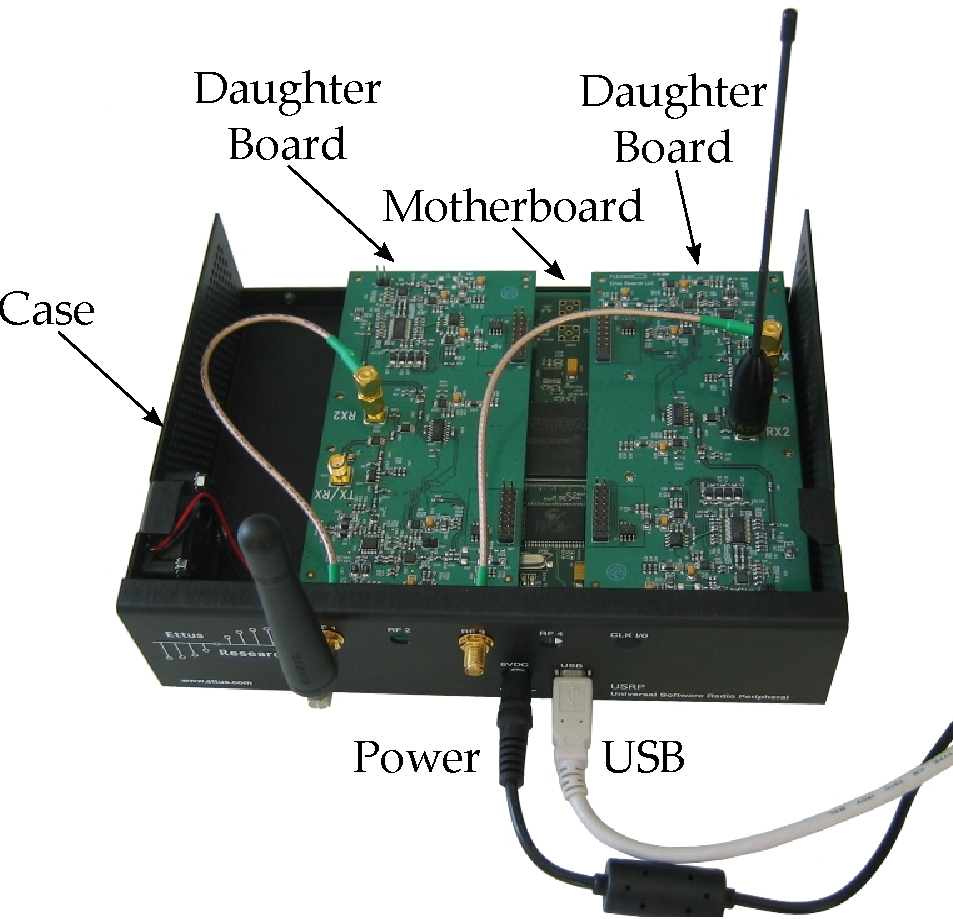
\includegraphics[width=0.8\textwidth]{../kapitel03/figures/USRP_DB_small.pdf}
%	\caption{The USRP motherboard equipped with two daughter boards}
%	\label{fig:USRP_photo}
%\end{figure}
%
%\subsection{The USRP Motherboard}
%The motherboard is equipped with a Cyclone EP1C12 FPGA from Altera \cite{altera_cyclone}, which provides the interfaces to the \ac{USB} and to the \acp{ADC} and \acp{DAC}. Two \acp{ADC} and two \acp{DAC} are integrated in a single AD9862 \cite{ad9862} conversion chip. Due to the fact that the board is equipped with two AD9862, the motherboard provides a total of four transmit and four receive paths. The \acp{ADC} support a sample rate of \SI{64}{MHz} with a quantization resolution of \SI{12}{bit}. Furthermore they provide \acp{PGA}, bypassable low pass decimation filters and a bypassable Hilbert filter. The transmit side of the AD9862 provides two \SI{128}{MHz} \acp{DAC} with \SI{14}{bit} resolution as well as interpolation filters and digitally tunable real or complex up-converters.
%
%Figure \ref{fig:USRP_motherboard} shows the motherboard in more details. The \ac{FPGA} is located at the center of the board and the two ADC/DAC combinations are in adjacency on the right and left side. The chip, shown in figure \ref{fig:USRP_motherboard}, below the FPGA is a Cypress' FX2 \ac{USB} microcontroller \cite{cypress_fx2}, which supports the connection to the \ac{USB} peripheral. The white plug-ins over and under the AD9862 conversion chips are the connectors to the daughter boards.
%
%\begin{figure}
%	\centering
%	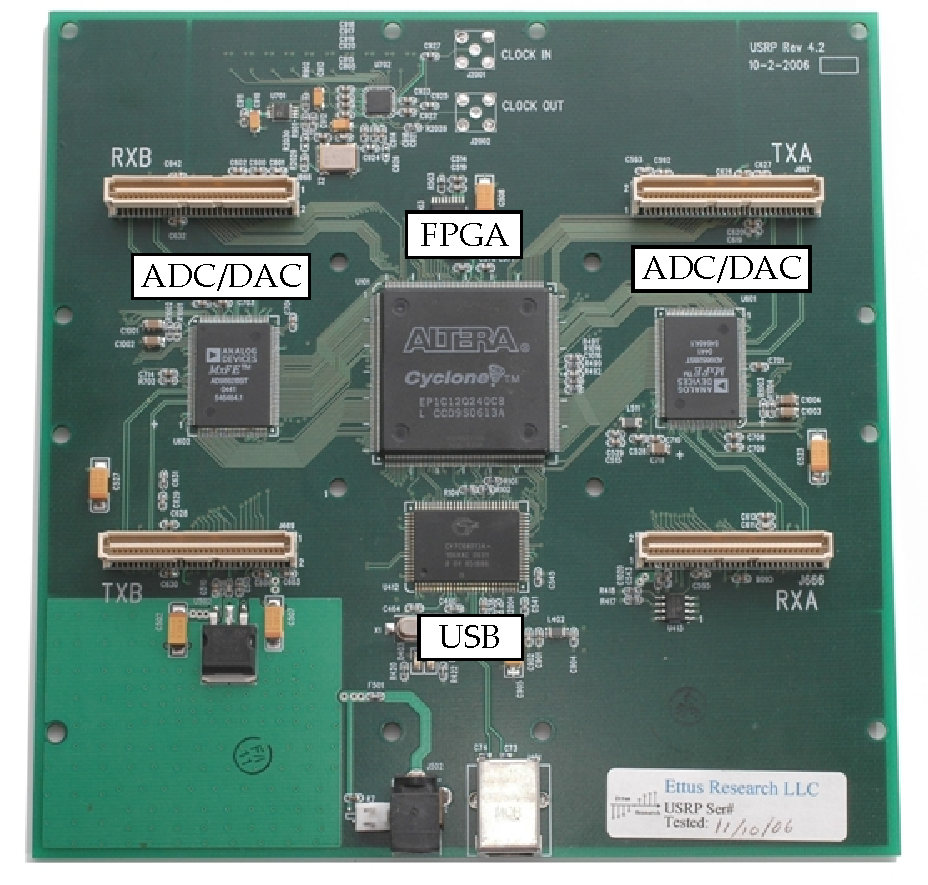
\includegraphics[width=1.0\textwidth]{../kapitel03/figures/USRP_MB_small.pdf}
%	\caption{The USRP motherboard \cite{ettus:website}}
%	\label{fig:USRP_motherboard}
%\end{figure}
%
%\subsection{The USRP Daughter Boards}
%\label{subsec:USRP_DB}
%Ettus Research provides a variety of daughter boards for the \ac{USRP}, working in a frequency range from baseband up to  \SI{5}{GHz}. In this subsection only the Flex400\index{Flex400} and Flex2400\index{Flex2400} daughter boards are described. These front ends were used for the implemented waveforms in chapter \ref{chapter:wf} and chapter \ref{chap:further}.
%
%The Flex400 supports a frequency range from \SI{400}{MHz} to \SI{500}{MHz} while the Flex2400 is designed for RF signals between \SI{2400}{MHz} and \SI{2500}{MHz}. Other  \ac{USRP} daughter boards are described in \cite{ettus:website}. The Flex400 and Flex2400 are designed similarly in a way that they are using a single conversion topology for upconversion and downconversion.
%
%For the Flex400, the received signal is sent to the AD8348 direct quadrature demodulator \cite{ad8348}. The demodulator needs a carrier for mixing the RF signal into baseband. This signal comes from a \ac{VCO}/\ac{PLL} combination, which is able to tune the frequency in steps of \SI{4}{MHz}. This does not achieve an exact direct-conversion architecture but results in a low IF topology, where the intermediate frequency varies between baseband and \SI{4}{MHz}. The last step for downconversion of the in-phase and quadrature components into baseband is done on the motherboard inside the FPGA with a Digital Down Converter (DDC).
%
%The architecture of the Flex2400 is equal but an AD8347 \cite{ad8347} quadrature modulator replaces the AD8348 due to the higher frequency range. The receiver structure is shown in figure \ref{fig:signal_flow_USRP}. The Anti-aliasing filter is the same for both daughter boards and comprises resistances, capacitors and inductors with known values due to the open source schematics. The transfer function was calculated and is shown in figure \ref{fig:transfer_function_flex400}. The 6 dB cut off frequency is at \SI{22}{MHz}.
%
%\begin{figure}
%\centering
%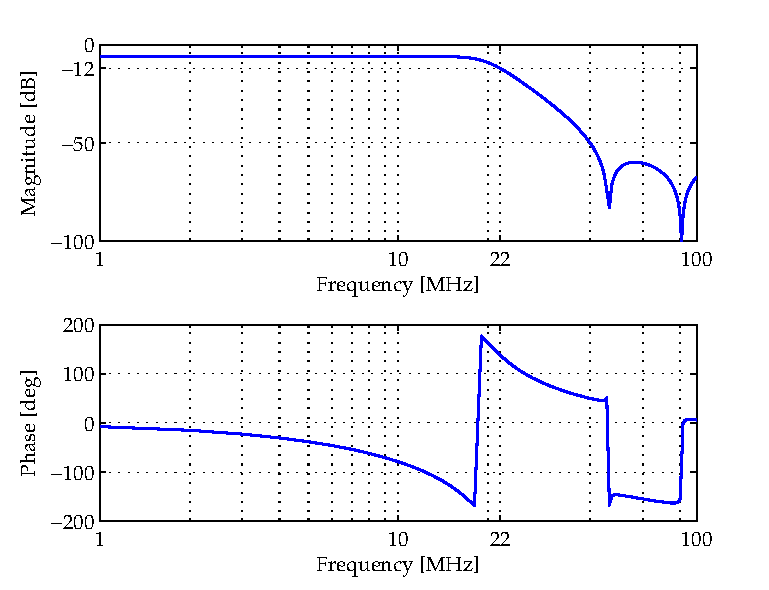
\includegraphics[width = 1.0\textwidth]{../kapitel03/figures/transfer_function_flex400.pdf}
%\caption{Transfer function of the anti-aliasing filter for the Flex400 and Flex2400 daughter boards}
%\label{fig:transfer_function_flex400}
%\end{figure}
%
%The transmit path is designed analogically to the receive path as shown in figure \ref{fig:signal_flow_USRP}. The AD8345 quadrature modulator \cite{ad8345} converts the signals to a radio frequency between \SI{400}{MHz} and \SI{500}{MHz} for the Flex400. The local oscillator is the same version as for the receive path, where digital up conversion of the baseband signal to an intermediate frequency between baseband and \SI{4}{MHz} is necessary. This can be done with the internal Digital Up Converter in the AD9862 \cite{ad9862}. The difference between Flex2400 and Flex400 daughter board is again the different frequency range of the modulator.
%
%
%\subsection{Platform Specific Constraints}
%
%Figure \ref{fig:signal_flow_USRP} shows a signal flow graph for a software radio platform with a Flex400/Flex2400 front end. As described before, both daughter boards have the same structure but with different modulators and demodulators as well as different VCO/PLL combinations. The USRP motherboard works as a conversion module. Custom signal processing can be implemented either on the FPGA or on the GPP respectively.
%
%\begin{table}
%	\centering
%		\begin{tabular}{|c||c|c|}
%		\hline
%		\multirow{2}{*} {EP1C12} & \multicolumn{2} {|c|}{Logic Elements}\\
%				&	12060 &	100 \% \\
%		\hline
%		Tx				&	1214	&	10 \%	\\
%		Rx				&	3448	&	29 \% \\		
%		Tx \& Rx	&	3895	& 32 \% \\
%		\hline
%		\end{tabular}
%	\caption{Minimum number of Logic Elements used in the FPGA}
%	\label{tab:MinimumAmountOfLogicElementsUsedInTheFPGA}
%\end{table}
%
%Table \ref{tab:MinimumAmountOfLogicElementsUsedInTheFPGA} gives an overview how much space the \ac{FPGA} provides. Without any logic usage, Altera's Cyclone EP1C12 has a total of 12060 \acp{LE}. However, all these elements cannot be used for signal processing due to the fact that the interfaces to the AD9862 as well as buffers and interfaces to the USB chip have to be implemented. With the transmit and receive sides, approximately \SI{68}{\%} of the internal logic can be used for signal processing. The space occupancy for a receive only configuration is about three times higher than for a pure transmitter. This is due to the fact that in the receive side a \ac{DDC} has to be implemented. This is not the same for the transmit side, since the internal \ac{DUC} on the AD9862 can be used. These results are summarized in table \ref{tab:MinimumAmountOfLogicElementsUsedInTheFPGA}.
%
%Another platform specific limitation is the \ac{USB}\index{USB} connection between motherboard and \ac{GPP}. While USB 2.0 supports data rates up to \SI{480}{Mbps}, the USB controller from Cypress together with the library: \emph{libusb} on the GPP achieves a maximum throughput of \SI{228}{Mbps}. With this, a complex bandwidth of approximately \SI{7}{MHz} with \SI{16}{bit} wide in-phase and quadrature samples is achieved. To get the lower sample rate in comparison to the conversion rate of the ADCs, a decimation filter has to be implemented with a factor not less than eight on the receive side. On the transmit side an interpolation filter with an upsampling rate not less than four is necessary. These filters have to be implemented for in-phase and quadrature signal components.
%
%\begin{landscape}
%\begin{figure}
%    \centering
%    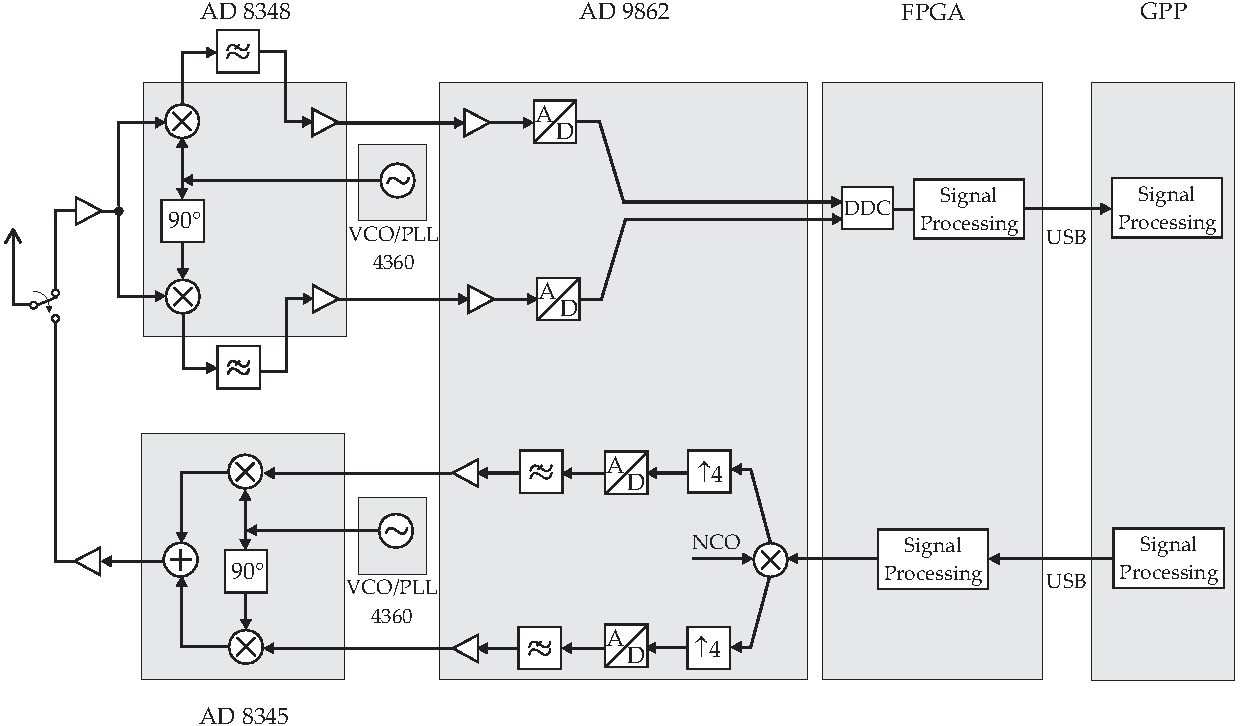
\includegraphics[width=1.4\textheight]{../kapitel03/figures/signal_flow_USRP.pdf}
%    \begin{flushright}
%    \caption{Signal flow in a USRP}
%    \label{fig:signal_flow_USRP}
%    \end{flushright}
%\end{figure}
%\end{landscape}
%
%\subsection{Integration in the design flow}
%
%\subsubsection{Integration of the FPGA}
%
%%Figure \ref{fig:USRP_FPGA_Black_Box} gives an overview of the FPGA, where it should be highlighted that the baseband data are coming from the ADC and are passing to the DAC with fixed data rates and word lengths. Therefore, on the receive side a \ac{DDC} is implemented that can be configured through a register by the \ac{GPP}. As mentioned previously, a \ac{DUC} is already included at the transmit side on the \ac{DAC}. The \emph{Rx Chain} and \emph{Tx Chain} blocks are black boxes with interfaces to in-phase and quadrature signal components as well as to the clock. This makes the integration of the generated Verilog code possible. The generated time scopes inside the black boxes are connected automatically with buffers at the transmit or receive side of the \ac{USB}. In addition, interrupt commands for the GPP are provided in a form that the GPP can handle the sample rate. 
%
%
%%\begin{figure}[htbp]
%%	\centering
%%		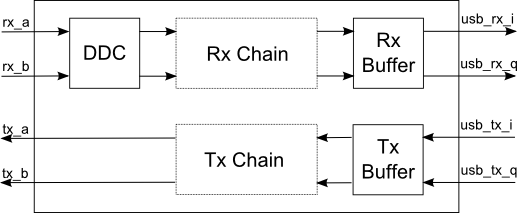
\includegraphics{../kapitel03/figures/USRP_FPGA_Black_Box.pdf}
%%	\caption{Black boxes in the FPGA on the USRP}
%%	\label{fig:USRP_FPGA_Black_Box}
%%\end{figure}
%
%
%The transformation from \ac{PSM} to the raw binary file for the FPGA is presented in figure \ref{fig:codegener_FPGA_USRP}. The functional code is generated from the \ac{PSM}. This is the code that is integrated in the \emph{RX Chain} at the receive path and in the \emph{TX Chain} at the transmit path. A template makefile, written in \ac{TCL}, is doing the synthesizing and mapping of the code. It includes information concerning the FPGA, the synthesizer and mapper as well as the physical connections to the chip. Additional Verilog code for the platform specific functions like buffers are integrated in the development flow. The resulting file can be uploaded to the FPGA.  
%
%\begin{figure}[htbp]
%	\centering
%		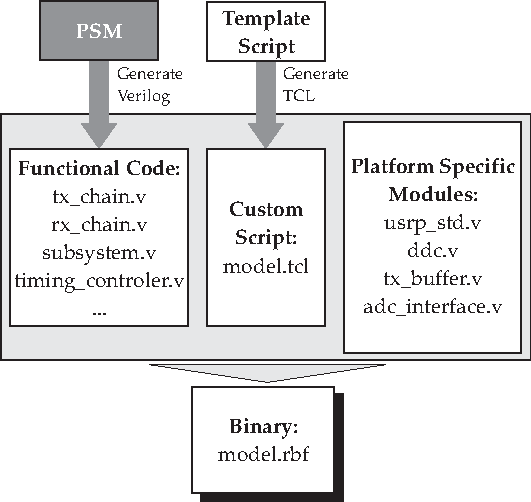
\includegraphics{../kapitel03/figures/codegener_FPGA_USRP.pdf}
%	\caption{Transformation from the \ac{PSM} to the bitstream on the Cyclone FPGA}
%	\label{fig:codegener_FPGA_USRP}
%\end{figure}
%
%
%\subsubsection{Integration of the GPP}
%The integration of the GPP is done by implementing an interface which is based on the USRP API from GNU Radio. This interface must be extended for code generation and inclusion in Simulink. Therefore two APIs are build: a \texttt{usrp\_source} object that handles the data transfer from the USRP to the GPP and a \texttt{usrp\_sink} object that handles the connection from GPP to USRP. Figure \ref{fig:usrp_sink_source} shows these interfaces in the Simulink\index{Simulink} environment.
%
%\begin{figure}[htbp]
%	\centering
%		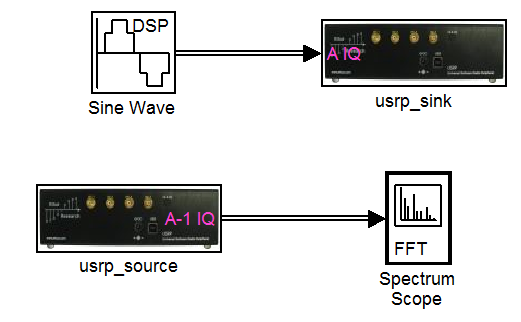
\includegraphics[width=0.6\textwidth]{../kapitel03/figures/usrp_sink_source.PNG}
%	\caption{Example for the use of the APIs for integration of the USRP in a model}
%	\label{fig:usrp_sink_source}
%\end{figure}
%
%The interfaces are implemented such that for code generation, the platform specific objects are linked to the functional code. According to the example in figure \ref{fig:usrp_sink_source} the \texttt{usrp\_sink} receives the data from the sine wave and sends it to the USB buffer and then to the FPGA. The \texttt{usrp\_source} gets new data from the USB buffer and passes it to the spectrum scope. To maintain real time processing, the USRP sends interrupts when a new frame of data can be accessed in the USB buffer. An error is produced if these data are not used or not passed over before the next interrupt arrives. This \ac{ISR} controls the timing and the scheduling of the code running on the GPP.
%
%For configuring the data, a \ac{GUI} was developed shown in figures \ref{fig:usrp_sink_mask_usrp} and \ref{fig:usrp_sink_mask_subdev}. The parameters for timing and scheduling can be configured via the GUI shown in figure \ref{fig:usrp_sink_mask_usrp}. The \ac{ISR} time period $T_{\text{ISR}}$ can be calculated as follows:
%\begin{equation}
%	T_{\text{ISR}} = \frac{f_{DAC}}{I} \cdot N_{\text{frame}},
%\end{equation}
%where $f_{DAC}$ is the sampling rate of the DAC, $I$ is the interpolation factor and $N_{\text{frame}}$ is the vector length.
%This would lead to an \ac{ISR} time period of \SI{4.096}{ms} for the configuration shown in figure \ref{fig:usrp_sink_mask_usrp}.
% 
%
%\begin{figure}
%	\centering
%		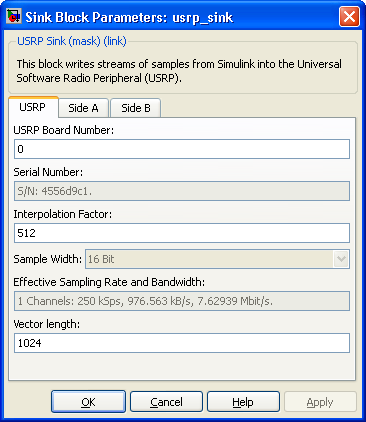
\includegraphics[width=0.75\textwidth]{../kapitel03/figures/usrp_sink_mask_usrp.png}
%	\caption{GUI for the USRP sink with an example for configuration parameters}
%	\label{fig:usrp_sink_mask_usrp}
%\end{figure}
%
%Figure \ref{fig:usrp_sink_mask_subdev} shows the configuration for the USRP daughter boards. The daughter board ID is  written to the text field and gives additional information like the maximum tuning frequency and the range of the gain. All these data are written to the APIs. The interfaces for the daughter board expect the tuning of the frequency and the gain as input data. Additionally, the data type can be configured as well as the selection of the antenna type through the antenna ID. The setting of the configuration can be done for both daughter boards by selecting one of the two tabs: \emph{Side A} or \emph{Side B}.
%
%
%\begin{figure}
%	\centering
%		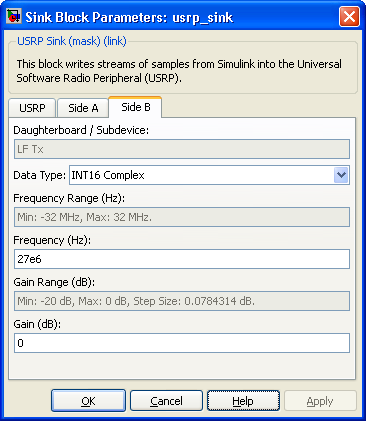
\includegraphics[width=0.75\textwidth]{../kapitel03/figures/usrp_sink_mask_subdev.png}
%	\caption{GUI for the USRP subdevice, showing configuration values}
%	\label{fig:usrp_sink_mask_subdev}
%\end{figure}
%
%Figure \ref{fig:codegener_GPP_USRP} gives an overview of the transformation from \ac{PSM} to executable code, according to the transformation from \ac{PSM} to bitstream shown in figure \ref{fig:codegener_FPGA_USRP}. As described in section \ref{sec:codegen}, the functional code is generated in a C++ code. With the integration of the \texttt{usrp\_sink} or \texttt{usrp\_source} objects, the functional code can be linked to the source code of the interfaces. The template makefile starts the development environment as well as the compiler and linker. The output is a file that can be executed on any host PC operating with Windows or Linux operating system. 
%
%\begin{figure}[htbp]
%	\centering
%		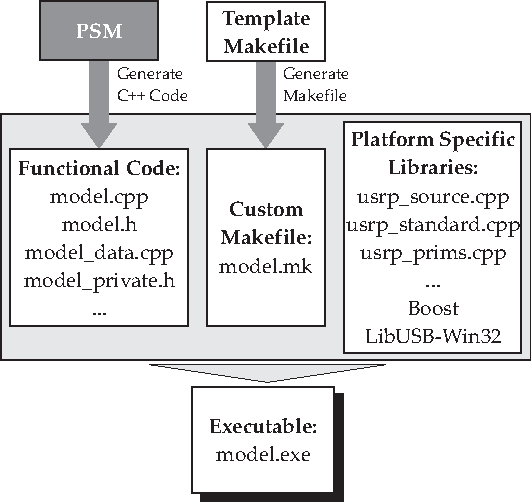
\includegraphics{../kapitel03/figures/codegener_GPP_USRP.pdf}
%	\caption{Transformation from the \ac{PSM} to an executable file for the GPP}
%	\label{fig:codegener_GPP_USRP}
%\end{figure}
%
%
%
%
%\section{Small Form Factor SDR}
%\label{sec:SFF}
%Lyrtech's \ac{SFF SDR DP} \cite{lyrtech_sff_sdr} was one of the first embedded development platforms for Software Defined Radios. The platform\index{Platform} was originally developed as an evaluation board for Texas Instrument's Da Vinci \ac{SoC}. Lyrtech used the processing power of the included processors for Software Radio applications and extended it with \acp{ADC}, \acp{DAC} and various RF front ends. The \ac{SFF SDR DP} consists of three modules, which are shown in figure \ref{fig:sff_sdr}. The \ac{DPM} is the signal processing layer at the bottom with a \ac{GPP}/\ac{DSP} combination in addition to an \ac{FPGA}. The \ac{DCM} is the middle layer and is equipped with an additional \ac{FPGA} for sample rate conversion as well as \acp{ADC} and \acp{DAC}. The Radio Frequency Module (RFM) finally is the RF front end on the top. 
%\begin{figure}
%	\centering
%		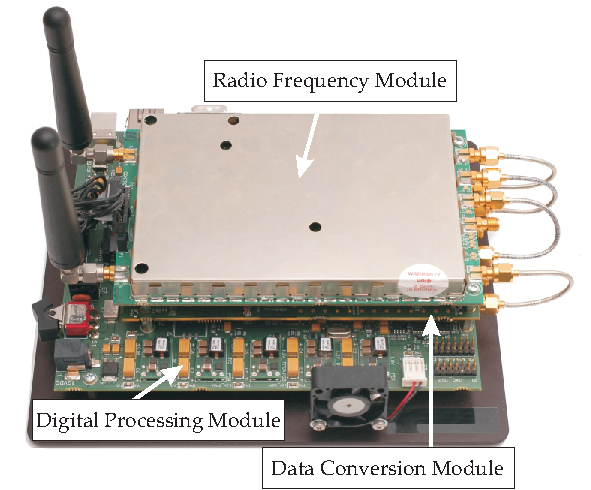
\includegraphics[]{../kapitel03/figures/sff_sdr.pdf}
%	\caption{Illustration of the SFF SDR DP, showing the three different modules}
%	\label{fig:sff_sdr}
%\end{figure}
%
%\subsection{Digital Processing Module (DPM)}
%\index{Digital Processing Module}
%As the name indicates, the whole signal processing on the SFF SDR is placed on the \ac{DPM}. Therefore, the board is equipped with a Virtex 4 SX35 FPGA \cite{virtex4} and TI's TMS320DM6446 \ac{SoC} \cite{ti_dm6446} as the central processing units. The \ac{SoC} comprises two processing cores: a C64x+ fixed point \ac{DSP} and an ARM \ac{GPP}. An overview of the architecture of the \ac{DPM} is given in figure \ref{fig:Digital_Processing_Modul}. The exact properties of the components are described in table \ref{tab:SFF_SDR_DPM}. The \ac{FPGA} and the \ac{DSP} are connected via the \ac{VPSS}. This is a 16-bit synchronous video data transfer port for the \ac{DSP}, which was originally designed as a video processing chip. The \ac{VPSS} was adapted to provide high data rates between both processing units with the \ac{VPFE} as the interface towards the DSP and the \ac{VPBE} in the opposite direction back to the FPGA. Both interfaces are independent from another. Furthermore, there are two additional connections between \ac{FPGA} and \ac{DSP}: The \ac{EMIF} allows access to read from and to write to registers, while the \ac{ASP} is connected to the on board PCM3008 audio stereo codec through the \ac{FPGA}. Beside the audio codec, the Virtex 4 allows access to several buttons, switches, LEDs and to the \ac{DCM} over a proprietary bus system. The peripherals of the DSP consists of the RS232 interface to configure the IP-address, the DDR2 RAM external memory with \SI{128}{MB} and a high speed USB bus, which is not supported by the firmware right now. Further peripheral equipments are an Ethernet connection for board access over a host PC, a slot for an SD card and another \SI{128}{MB} memory, which stores the bootloader and a kernel image of the operating system and the file system.
%
%
%\begin{table}
%	\centering
%		\begin{tabular}{|c|c||c|}
%		\hline
%		\multicolumn{3}{|c|}{ \textbf{TMS320DM6446 DMP SoC}} \\
%		\hline
%		\hline
%		\multicolumn{2} {|c||}{Core Frequency}	&	{\SI{594}{MHz}}\\
%		\hline
%		\multicolumn{2} {|c||}{Peak MMAcs}			&	{4752} \\
%		\hline
%		\multirow{2}{*}{On-chip L1/SRAM}	& DSP									& \SI{112}{kB} \\
%																			& GPP									&  \SI{40}{kB} \\
%		\hline
%		\multirow{2}{*}{On-chip L2/SRAM}	& DSP									&  \SI{64}{kB} \\
%																			& GPP									&   \SI{0}{kB} \\
%		\hline
%		ROM																& GPP 								&  \SI{16}{kB} \\
%		\hline
%		\multirow{2}{*}{EMIF}							& EMIFA								& \SI{16}{bit} / \SI{8}{bit} \\
%																			& DDR2								& \SI{32}{bit} / \SI{16}{bit} \\
%		\hline
%		\multirow{2}{*}{Timer}						& GP									& \SI{64}{bit} \\
%																			& WD									& \SI{64}{bit} \\
%		\hline
%		\hline		\multicolumn{3}{|c|}{ \textbf{Virtex 4 XC4VSX35 FPGA}} \\ 
%		\hline
%		\hline
%		\multicolumn{2} {|c||} {CLB array}							& 96x40	\\
%		\hline
%		\multicolumn{2} {|c||} {Slices}								& 15360 \\
%		\hline
%		\multicolumn{2} {|c||} {Block RAM bits (\#)} 	& 3456 (192) \\
%		\hline
%		\multicolumn{2} {|c||} {18 x 18 multpliers}		& 192 \\
%		\hline
%		\multicolumn{2} {|c||} {Digtal Clock Manager}										& 8 \\
%		\hline
%		\end{tabular}
%	\caption{Properties of the digital processing units on DPM}
%	\label{tab:SFF_SDR_DPM}
%\end{table}
%
%\begin{figure}[tbp]
%	\centering
%		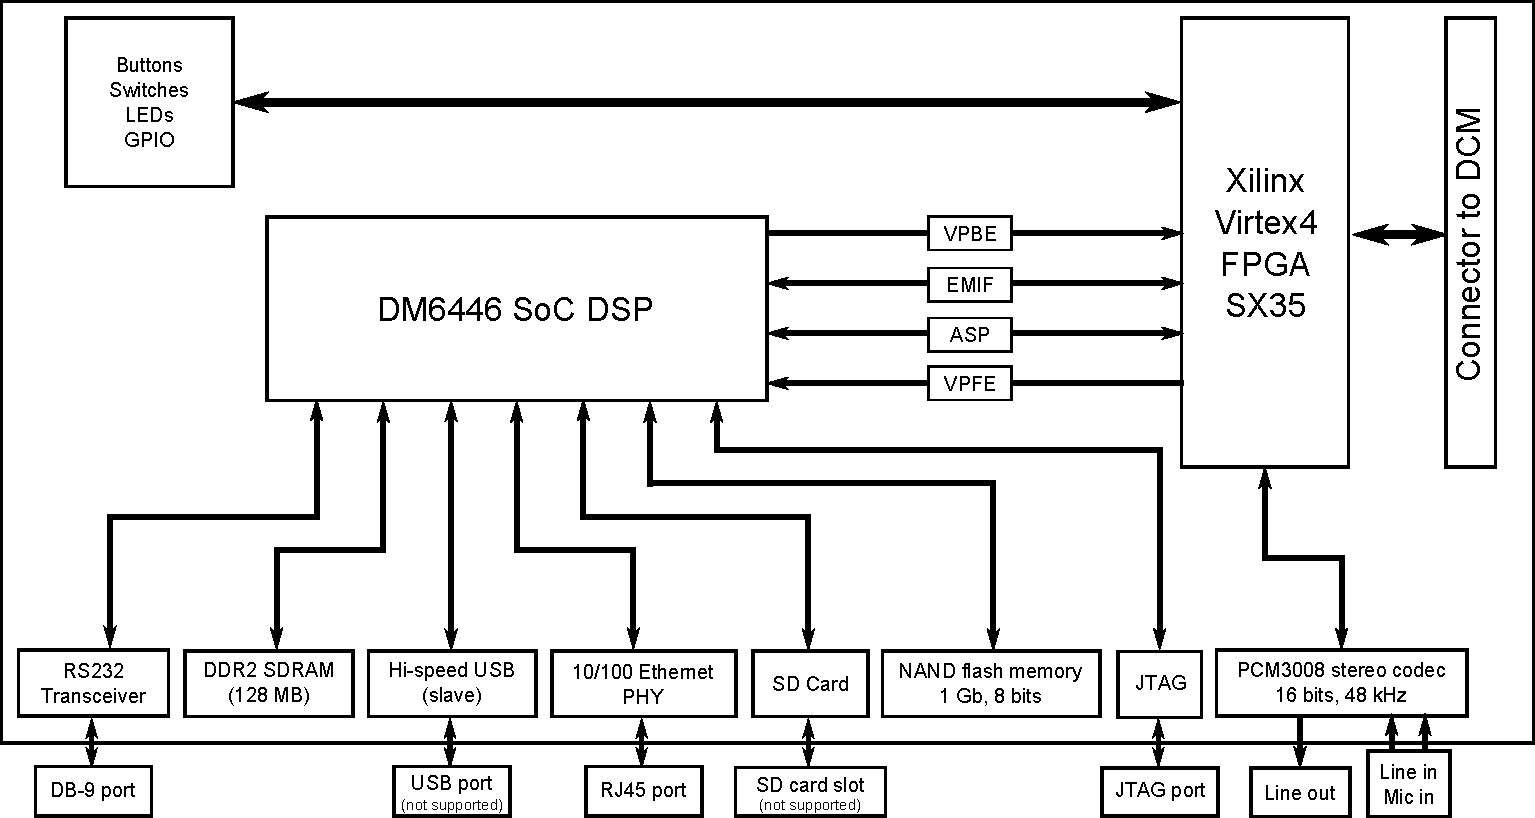
\includegraphics[width=1.0\textwidth]{../kapitel03/figures/Digital_Processing_Modul.pdf}
%	\caption{Structure of the Digital Processing Module}
%	\label{fig:Digital_Processing_Modul}
%\end{figure}
%
%\subsection{Data Conversion Module (DCM)}
%\index{Data Conversion Module}
%\begin{figure}[tbp]
%	\centering
%		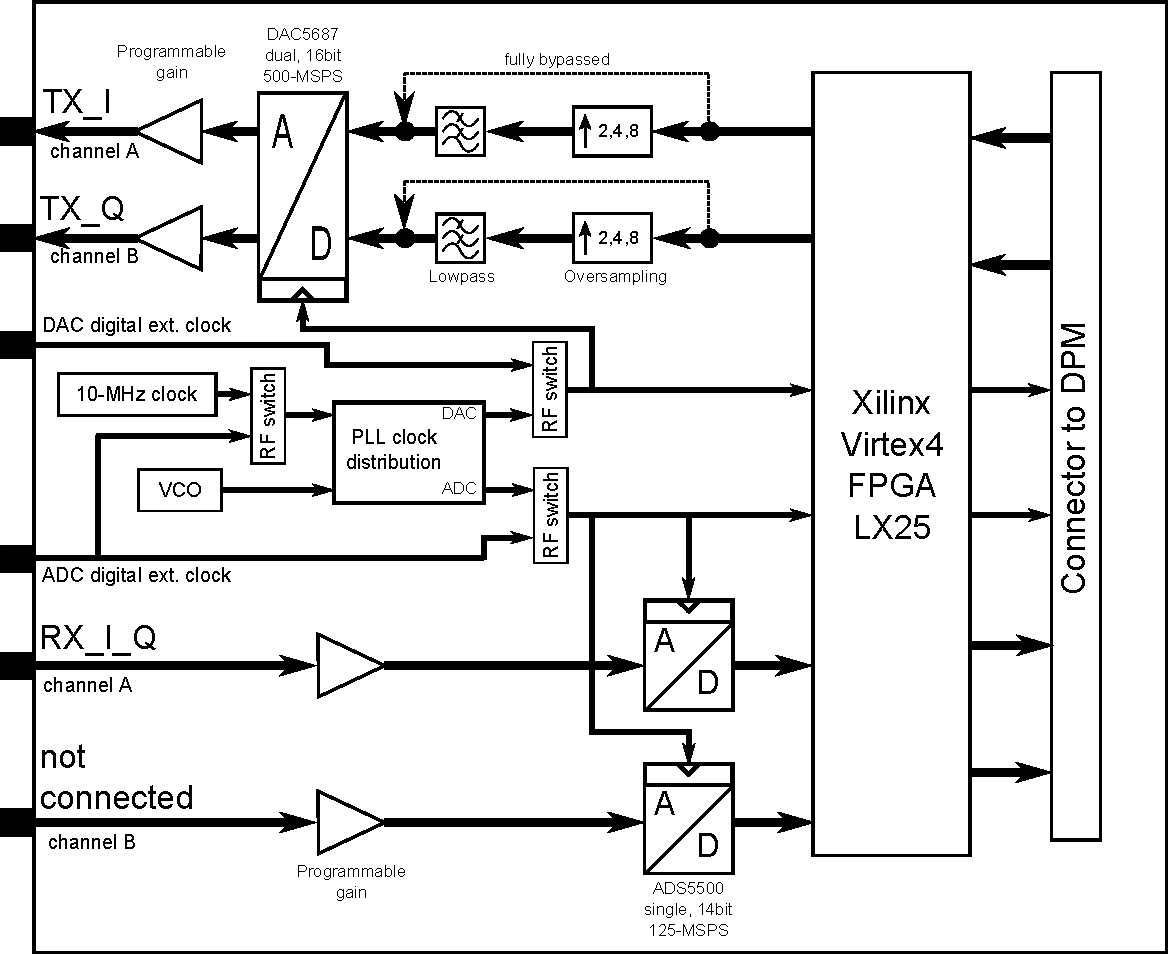
\includegraphics[width=1.00\textwidth]{../kapitel03/figures/Data_Conversion_Modul.pdf}
%	\caption{Structure of the Data Conversion Module}
%	\label{fig:Data_Conversion_Modul}
%\end{figure}
%
%The \ac{DCM} is the interface between the digital world of the \ac{DPM} and the analog RF front end. The DCM is equipped with two \acp{ADC}, two \acp{DAC}, an \ac{FPGA} and a clock distribution unit. The \ac{ADC} is a Texas Instruments ADS5500 \acl{ADC} \cite{ads5500} with a maximum sampling frequency of \SI{125}{MHz} and a resolution of \SI{14}{bit}. As shown in figure \ref{fig:Data_Conversion_Modul}, two ADS5500 are needed for a complex baseband signal received from a direct-conversion receiver. This is different to the \acp{RFM} described in section \ref{subsec:RFM}, where the incoming signal on an \ac{IF} on \SI{30}{MHz} or \SI{44}{MHz} is real. Therefore, the second input port and the second \ac{ADC} is not used. After sampling, the digitized data are passed to Xilinx's Virtex-4 LX25 \ac{FPGA}, which is the interface between the conversion chips and the proprietary expansion connector. This \ac{FPGA} here is not designated for custom signal processing and its logic cannot be changed.
%
%The transmit side of the board consists mainly of \ac{TI}'s DAC5687 Dual\--Chan\-nel \ac{DAC} \cite{dac5687}. This chip comprises two \acp{DAC} with a bit resolution of 16 at a maximum sampling rate of \SI{500}{MHz}. Furthermore, it provides an interpolation filter for upsampling by a factor of 2, 4 or 8, as well as a complex modulator and a programmable amplifier. 
%
%The clock of the \ac{DCM} controls the sample rate converters. It is based on Analog Device's AD9511 \ac{PLL} \cite{ad9511}. The reference clock for the \ac{PLL} is supported from the on-board \SI{10}{MHz} internal \ac{LO} or from an external clock. With the limited frequency range from \SI{800}{MHz} to \SI{1400}{MHz} of the \ac{VCO}, the target clock frequency $f_{out}$ can be calculated by
%\begin{equation}
%	f_{\textnormal{out}} =  \frac{f_{\textnormal{VCO}}}{\text{div}} = \frac{N}{R\cdot \text{div}}\cdot f_{\textnormal{ref}}\; .
%	\label{eq:f_out_PLL}
%\end{equation}
%In equation (\ref{eq:f_out_PLL}), div is the clock divider, which is realized as a 5-bit counter. This leads to a division range of $[1\dots32]$. $R$ is the \ac{PLL} reference divider with a division range between one and 16383 due to the implemented 14-bit counter. The feedback divider $N$ is a combination of a 3-bit prescaler and two counters $A$ (\SI{6}{bit}) and $B$ (\SI{13}{bit}). Through combinations in the prescaler, any integer value for $N$ in the range of $[1\dots262112]$ can be selected.
%Figure \ref{fig:f_out_pll} gives an example for the possible division factors between $N$ and $R$ with a given reference \ac{LO} at \SI{10}{MHz}. Due to the limitations of the \ac{VCO} in the interval between \SI{800}{MHz} to \SI{1400}{MHz}, the ratio between feedback and reference divider is limited to
%\begin{equation}
%	\frac{N}{R} =  \frac{f_{\textnormal{VCO}}}{f_{\textnormal{ref}}} = [80 \dots 140] \;.
%	\label{eq:frac_N_R}
%\end{equation}
%These are the upper and lower bounds for the ratio, shown in figure \ref{fig:f_out_pll}. The curves represent any possible value for the clock divider div. The remaining parameters can finally be chosen as follows:
%\begin{equation}
%	\frac{N}{R} =  \frac{P\cdot B+A}{R}
%	\label{eq:frac_N_R_2}
%\end{equation}
%With this clock distribution circuit any sampling frequency with high accuracy can be achieved. Therefore no more complex resampling algorithms have to be implemented on the \ac{FPGA} or on the \ac{DSP} to provide the system's base sampling rate.
%
%\begin{figure}
%	\centering
%		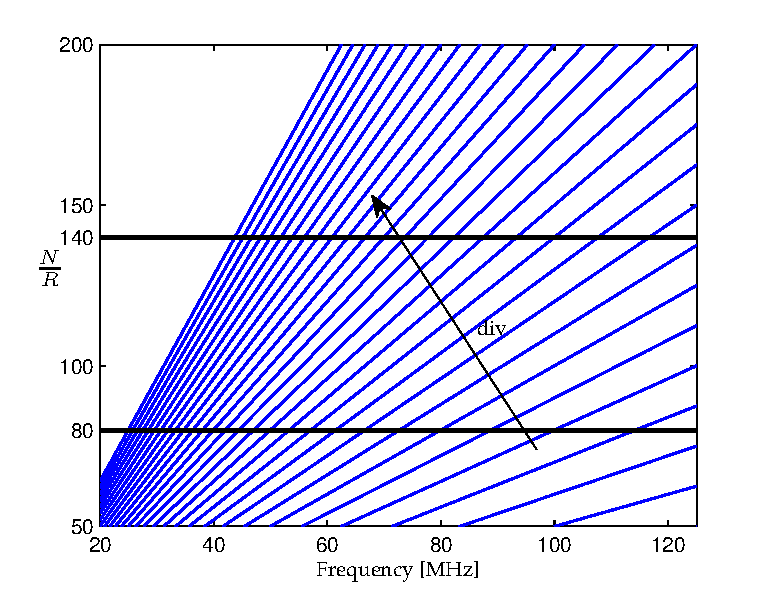
\includegraphics[width = 1.0\textwidth]{../kapitel03/figures/f_out_pll.pdf}
%	\caption{Ratios between $N$ and $R$ over the target frequency for different divider values div}
%	\label{fig:f_out_pll}
%\end{figure}
%
% 
%\subsection{Radio Frequency Module}
%\label{subsec:RFM}
%In the following two subsections the Tunable Low Band RF module and the WiMAX RF module are described. These two modules are used in conjunction with the \ac{SFF SDR DP}.
%
%\subsubsection{Tunable RF Module}
%\index{Tunable RF Module}
%
%\begin{figure}
%	\centering
%		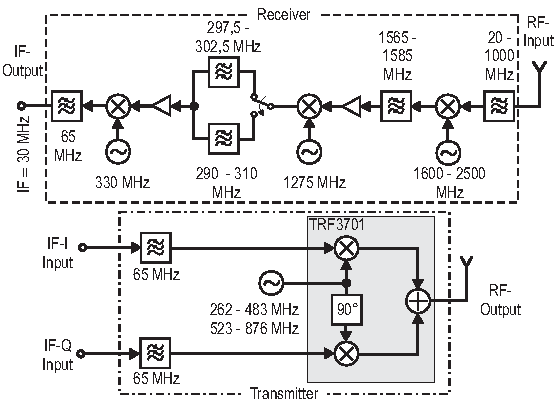
\includegraphics[width=1.00\textwidth]{../kapitel03/figures/Tunable_RF_Module.pdf}
%	\caption{Structure of the Tunable RF Module}
%	\label{fig:Tunable_RF_Module}
%\end{figure}
%
%The Tunable RF module consists of a superheterodyne receiver\index{Superheterodyne receiver} with three stages, which converts signals between \SI{200}{MHz} and \SI{1}{GHz} to an \ac{IF} of \SI{30}{MHz}\index{Intermediate frequency}. It is equipped with five analog filters and three local oscillators. The first filter, close to the antenna, is a low-pass filter that suppresses all frequencies above \SI{1}{GHz}. The following \ac{LO} is a combination of \ac{PLL} and \ac{VCO}, which supports frequencies between \SI{1775}{MHz} and \SI{2575}{MHz} and converts the RF signal to a fixed frequency of \SI{1575}{MHz}. This is the center frequency of the second \SI{20}{MHz} wide bandpass filter. With a switch, two filters with different signal bandwidths of \SI{5}{MHz} or \SI{20}{MHz} can be selected. These bandpass filters have a center frequency of \SI{300}{MHz}. Before the bandpass filters, the signal is down converted with the second \ac{LO} with a mixing frequency of \SI{1275}{MHz}. The last step to an \ac{IF} of \SI{30}{MHz} is achieved with the third conversion stage of \SI{330}{MHz} and the final low pass filter for the images.
%
%The transmit side of the RF front end is built according to a direct-conversion transmitter, using TI's quadrature modulator TRF3701 \cite{trf3701}. An in-phase and a quadrature signal are mixed with the incoming signal from the \ac{LO}, which is composed of a \ac{PLL}, a \ac{VCO} and a didivide-by-two prescaler. In case when the prescaler is activated, a frequency of \SI{262}{MHz} up to \SI{483}{MHz} is generated while a frequency of \SI{523}{MHz} up to \SI{876}{MHz} is generated when the prescaler is deactivated.
%
%\subsubsection{WiMAX RF Module}
%\index{WiMAX RF Module}
%\begin{figure}
%	\centering
%		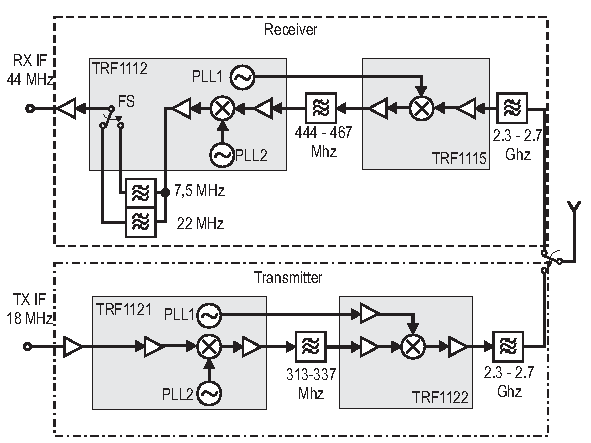
\includegraphics[width=1.00\textwidth]{../kapitel03/figures/WiMax_RF_module.pdf}
%	\caption{Structure of the WiMAX RF Module}
%	\label{fig:WiMax_RF_module}
%\end{figure}
%
%Similar to the Tunable RF module, the WiMAX RF module is a superheterodyne receiver\index{Superheterodyne receiver}. The supported frequency range of the front end is from \SI{2.3}{GHz} to \SI{2.7}{GHz}. This is also the frequency range for the wireless communication standard WiMAX. However, the WiMAX RF module has no bearing with the WiMAX specification but the frequency range. It converts signals from the \ac{RF} over two stages to an \ac{IF} of \SI{44}{MHz}. As shown in figure \ref{fig:WiMax_RF_module}, most components are integrated in \acp{IC}. The RF signal is limited by a \SI{400}{MHz} wide bandpass filter working on \SI{2.5}{GHz}. The first downconversion is done by \ac{TI}'s TRF1115 \cite{trf1115} low-noise down converter. It mixes the signal with an incoming carrier on a fixed frequency of \SI{456}{MHz}. On this frequency, the signal is filtered by a bandpass with a bandwidth of \SI{24}{MHz}. The final conversion on the \ac{IF} to \SI{44}{MHz} is done by a combination of \ac{PLL} and \ac{IF} down-converter (TRF1112 \cite{trf1112}) and is followed by the last filtering on a bandwidth of \SI{7}{MHz} or \SI{22}{MHz}. These last bandpass filters are switchable and controlled by TRF1112.
%
%The transmit side of the WiMAX RF module is designed as a two stage architecture composed of two \acp{IC} and two bandpass filters similar to the receive side architecture. The first up-converter (TRF1121 \cite{trf1121}) expects the transmit signal on a \SI{18}{MHz} \ac{IF} and mixes it up to a fixed frequency of \SI{325}{MHz}. Furthermore, it works as a \ac{LO} distributor for the second upconversion stage, where the mixing on frequencies between \SI{2.3}{GHz} and \SI{2.7}{GHz} is done (TRF1122 \cite{trf1122}). The bandpass filter between the upconversion stages limits the signal to a bandwidth of \SI{24}{MHz}, while the last bandpass filter on \SI{2.5}{GHz} limits the frequency on a  bandwidth of \SI{400}{MHz}.
%
%\subsection{Platform Specific Constraints}
%The C64x+ DSP is one of the processing units for the SFF SDR DP. This is in contrast to the USRP concept, where any GPP with an operating system can be used as a processing unit. With a clock frequency of \SI{594}{MHz}, the \ac{DSP} runs very fast, but the memory space for the signal processing code is limited to approximately \SI{176}{kB}. Code lengths that exceed this size have to be partitioned and moved to the external \ac{SDRAM}. Although it is dimensioned with a size of \SI{128}{MB}, the access time for read and write operations takes several cycles. This can slow down the running code until violating the real time constraints.
%
%Another limit for waveform development on the platform is the interface between \ac{DSP} and \ac{FPGA}. Originally intended to connect the processor to video peripherals, the \ac{VPSS} was rebuilt for data transfers from and to the \ac{FPGA}. With the underlying firmware it is not possible to achieve higher data rates than \SI{64}{Mbps}. This yields to a bandwidth of \SI{2}{MHz} assuming \SI{16}{bit} wide in-phase and quadrature components. Waveforms with higher bandwidths have to be processed on the \ac{FPGA}.
%
%As shown in table \ref{tab:SFF_SDR_DPM}, the Virtex4 provides 15360 slices and 192 multiplier components. Similar to the platform constraints for the \ac{USRP}, shown in table \ref{tab:MinimumAmountOfLogicElementsUsedInTheFPGA}, not all logic cells can be used for waveform development. Table \ref{tab:SFF_Virtex} summarizes the number of logic cells for different RF modules for the following configurations: single transmitter, single receiver or transceiver. It is remarkable that approximately \SI{15}{\%} of the resources are used for internal logic. This is due to the implementation of several \ac{FIFO} queus for the \ac{VPFE}, \ac{VPBE}, \ac{ADC} and \ac{DAC}. These buffers are built independently of the actual existence of a transmit or receive side. Further logic resources are used to implement the \ac{OPB} subsystem which provides access to the different peripherals. The differences for transmit and receive paths are due to the archiecture of the connected front end. The receive signal from the tunable RF module is a real signal on a \SI{30}{MHz} \ac{IF}. This makes downconverting and the implementation of a \ac{DDS} and two multipliers necessary. For the transmit side, a quadrature modulator is necessary on the tunable front end. The transmit side for the WiMAX module expects a real signal on \SI{18}{MHz} \ac{IF}. In this case upconversion and quadrature modulation have to be implemented on the \ac{FPGA}.
%
%\begin{table}
%	\centering
%		\begin{tabular}{|c|c||c|c|c|c|}
%		\hline
%		\multicolumn{2} {|c||} {\multirow{2}{*} {Virtex 4 SX35}} & \multicolumn{2} {c|}{Slices}			&	\multicolumn{2} {c|}{Multipliers} \\
%		\multicolumn{2}{|c||}{}																& 15360	& 100\%											& 192	& 100\%	\\
%		\hline
%		\multirow{3}{*}{WiMAX RF}					& TX								& 1942	& 12\%	 										& 7		& 3\% \\
%																			& RX								& 1981	& 12\% 											& 7	  & 3\% \\
%																			& TX \& RX					& 2046	& 13\%	 										& 9		& 4\% \\
%		\hline
%		\multirow{3}{*}{Tunable RF}				& TX								& 1907	& 12\% 											& 5 	& 2\% \\
%																			& RX								& 1981	& 13\%											& 7		& 3\% \\
%																			& TX \& RX					& 2016	& 13\% 											& 7		& 3\% \\
%		\hline
%		\end{tabular}
%	\caption{Space occupation with different RF modules and transmit receive configurations}
%	\label{tab:SFF_Virtex}
%\end{table}
%
%\subsection{Integration in the design flow}
%\subsubsection{Integration of the FPGA}
%Similar as for the USRP flow, the code generated for the \ac{PSM} is integrated in the existent environment. Figure \ref{fig:sff_fpga} gives an overview of the FPGA environment in the SFF SDR. The custom logic can be seen as a black box for the individual signal processing functions. Therefore, it provides interfaces to the data converters and to the \ac{VPSS} buses. Additional interfaces are for registers, interrupts and control strobes.
%
%\begin{figure}[htbp]
%	\centering
%		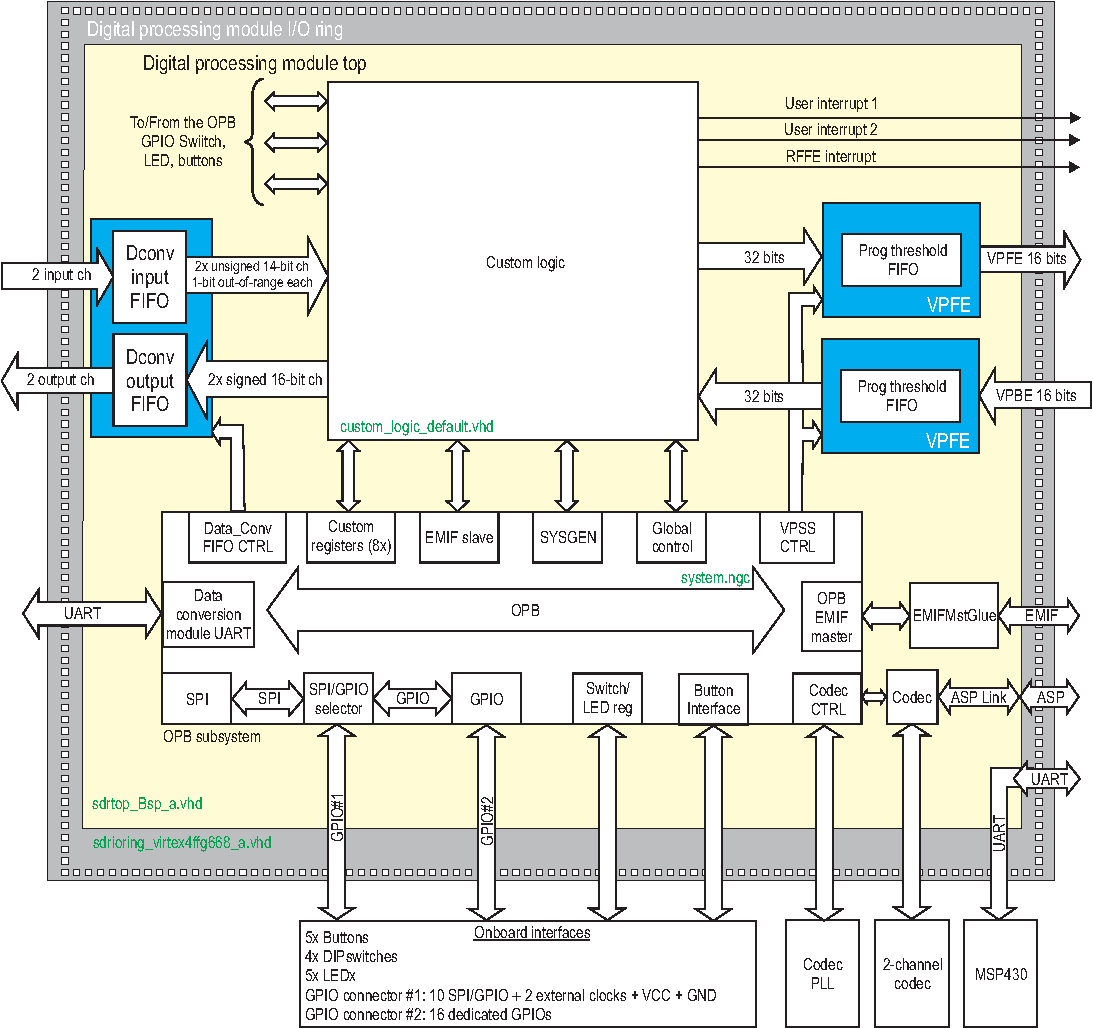
\includegraphics[width=1.00\textwidth]{../kapitel03/figures/sff_fpga.pdf}
%	\caption{Default configuration of the FPGA as in \cite{lyrtech_sff_sdr}}
%	\label{fig:sff_fpga}
%\end{figure}
%
%The transformation from \ac{PSM} to bitstream is shown in figure \ref{fig:codegener_FPGA_SFF_SDR}. The functional VHDL code is generated such that the interfaces to the data and control ports are connected automatically. The template makefile includes the entities and connects them with the provided netlists for the data buses and the additional platform specific functions. Furthermore physical properties and connections are given in the makefile that finally scripts the synthesizing and mapping of the code to a bitstream.
%
%\begin{figure}[htbp]
%	\centering
%		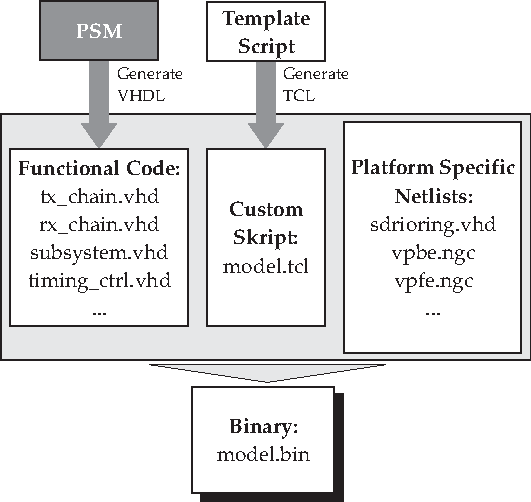
\includegraphics{../kapitel03/figures/codegener_FPGA_SFF_SDR.pdf}
%	\caption{Transformation from the \ac{PSM} to the bitstream on the Virtex4 FPGA}
%	\label{fig:codegener_FPGA_SFF_SDR}
%\end{figure}
%
%
%\subsubsection{Integration of the DSP}
%
%The integration of the \ac{DSP} in the design flow is done with APIs that connect the model with the data buses. An example of these APIs in the Simulink nevironment is shown in figure \ref{fig:SFF_DSP_API}. The interface to the \ac{VPSS} is implemented as a single block, where in the example of figure \ref{fig:SFF_DSP_API} a block in transmit direction is shown. The \ac{VPFE} interfaces are linked after code generation and compiling. The other platform specific interfaces are for configuration of the following modules: DSP, \ac{DCM} and \ac{RFM}. The configuration of the \ac{DSP} consists of building properties and arguments for the compiler. In contrast to the data conversion section on the \ac{USRP}, an own parametrization is needed for the \ac{DCM} to distribute the clock frequency or to adjust the gain. The configuration of the front end is similar to the USRP: the important parameters are the carrier frequency and the cutting frequencies of the bandpass filters. 
%
%\begin{figure}[htbp]
%	\centering
%		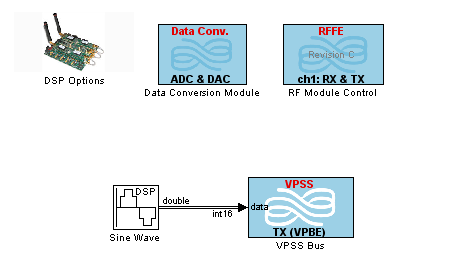
\includegraphics[width=0.85\textwidth]{../kapitel03/figures/SFF_DSP_API.PNG}
%	\caption{Example of the use of the APIs for the integration of the DSP on the \ac{SFF SDR DP}}
%	\label{fig:SFF_DSP_API}
%\end{figure}
%
%Figure \ref{fig:codegener_DSP_SFF_SDR} shows the transformation from \ac{PSM} to executable code, which is similar to the transformation shown in figure \ref{fig:codegener_GPP_USRP}. In this transformation the C code is generated and linked to the buses and APIs. The resulting code is compiled with the vendor specific development environment (Code Composer Studio) and loaded on the platform.
% 
%\begin{figure}[htbp]
%	\centering
%		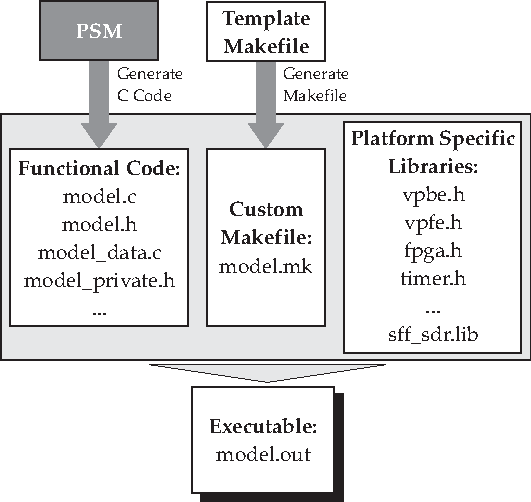
\includegraphics{../kapitel03/figures/codegener_DSP_SFF_SDR.pdf}
%	\caption{Transformation from the \ac{PSM} to the executable file for the DSP}
%	\label{fig:codegener_DSP_SFF_SDR}
%\end{figure}
%
%
